% ============================================================================
%  COMPILE WITH XeLaTeX  (twice, so the point total resolves)
%  Overleaf: Menu -> Compiler -> XeLaTeX
%  Requires: bnhandout.sty and fonts/Kalpurush.ttf in the project
% ============================================================================
\documentclass[11pt]{article}
\usepackage{bnhandout}          % add [nosol] for a student edition
\usepackage{hyperref}

\hauthor[https://sites.google.com/view/jugantordey/home]{Jugantor Dey}
\hseries{\textit{Mathematics for the Physics Olympiad}}

\begin{document}

\handouttitle{Chapter 14 : Limits}

\noindent
শুরু করার আগে ৪ নম্বর অধ্যায় থেকে domain, range ও piecewise ফাংশনের ধারণা,
আর ১০ নম্বর অধ্যায় থেকে $e^{x}$, $\ln x$ ও asymptote নিয়ে যা বলা হয়েছিল
সেটুকু দেখে নাও। ১৩ নম্বর অধ্যায়ের ছোট কোণের অসমতাটিও তৃতীয় অনুচ্ছেদে
সরাসরি লাগবে।

এই সিরিজে এতদিন যা করা হয়েছে তার প্রায় সবই ছিল বীজগণিত ও জ্যামিতি: সসীম সংখ্যক
ধাপে, নির্ভুলভাবে। এখান থেকে চরিত্র বদলাচ্ছে। ক্যালকুলাসের প্রতিটি ধারণা,
ডেরিভেটিভ হোক বা ইন্টিগ্রাল, একটি বাক্যের উপর দাঁড়িয়ে আছে: ``যত ছোট সম্ভব তার চেয়েও বেশি ছোট''।
আগের কয়েকটি অধ্যায়ে এই কথাটা কয়েকবার এসেছে এবং প্রতিবারই বলতে হয়েছে যে
এর নির্ভুল অর্থ পরে আসবে। এই অধ্যায়েই সেটা আসছে।

প্রথমেই একটা সতর্কবার্তা। limit-এর ধারণাটা কঠিন নয়, কিন্তু সহজ ভেবে দ্রুত পার
হয়ে গেলে পরে ডেরিভেটিভ কেবল সূত্র মুখস্থ হয়ে দাঁড়ায়। তাই এখানে ধীরে আগানোই ভালো;
বিশেষ করে ``$x \to a$ কিন্তু কখনোই $x = a$ নয়'' এই একটি কথা যতক্ষণ না রক্তে
মিশছে, ততক্ষণ পরের অধ্যায়ে যেয়ো না। এই অধ্যায়ে মোট \totalpoints\
পয়েন্ট আছে।

\section{লিমিট কী}

একটা সহজ প্রশ্ন দিয়ে শুরু করি। ধরো
\[
  f(x) = \frac{x^{2}-1}{x-1} .
\]
$x = 1$ বসালে $\dfrac{0}{0}$ আসে, যা অর্থহীন; অর্থাৎ $f$-এর domain-এ $1$ নেই।
কিন্তু $x$-কে $1$-এর কাছাকাছি নিলে কী হয়?

\begin{center}
\begin{tabular}{c|c|c|c|c|c|c}
 $x$ & $0.9$ & $0.99$ & $0.999$ & $1.001$ & $1.01$ & $1.1$ \\ \hline
 $f(x)$ & $1.9$ & $1.99$ & $1.999$ & $2.001$ & $2.01$ & $2.1$ \\
\end{tabular}
\end{center}

দুই দিক থেকেই মান $2$-এর দিকে যাচ্ছে। কারণটা বীজগণিতেই দেখা যায়: $x \neq 1$
হলে
\[
  \frac{x^{2}-1}{x-1} = \frac{(x-1)(x+1)}{x-1} = x+1 ,
\]
আর কাটাকাটির শর্তই হলো $x - 1 \neq 0$। সুতরাং $f$ আসলে $x+1$ ফাংশনটিই, কেবল
$x = 1$ বিন্দুতে একটি "ফুটো" বা বিচ্ছিন্নতা নিয়ে। ফুটোটা যেখানে, সেখানে ফাংশনের কোনো মান নেই;
তবু তার চারপাশে ফাংশনটির আচরণ পরিষ্কারভাবে $2$-এর দিকে ইঙ্গিত করছে।

\begin{idea}[Limit]
\[
  \lim_{x \to a} f(x) = L
\]
লেখার অর্থ: $x$-কে $a$-এর যথেষ্ট কাছে নিলে (কিন্তু $x = a$ না করে) $f(x)$-এর
মানকে $L$-এর যত কাছে ইচ্ছা আনা যায়।
\end{idea}

সংজ্ঞাটির প্রতিটি শব্দ গুরুত্বপূর্ণ, বিশেষ করে বন্ধনীর ভেতরের অংশটুকু।
$x \to a$ মানে $x$ ক্রমশ $a$-এর দিকে এগোচ্ছে, কখনো $a$ হচ্ছে না। তাই
$f(a)$-এর মান কী, এমনকি $f(a)$ আদৌ আছে কি না, তা limit-এর সঙ্গে সম্পর্কহীন।

তিনটি সম্ভাবনা ছবিতে দেখা যাক।

\begin{center}
\begin{tikzpicture}[x=1.0cm,y=1.0cm,>=stealth]
 \begin{scope}
  \draw[thick,->] (-0.3,0) -- (2.6,0) node[below] {$x$};
  \draw[thick,->] (0,-0.3) -- (0,3.1) node[left] {$y$};
  \draw[thick,domain=0.15:2.4,samples=60,variable=\x] plot ({\x},{0.8*\x+1});
  \draw[fill] (1,1.8) circle (2.2pt);
  \draw[dashed] (1,0) -- (1,1.8); \draw[dashed] (0,1.8) -- (1,1.8);
  \node[below] at (1,0) {$a$};
  \node at (1.3,-1.1) {(ক)};
 \end{scope}
 \begin{scope}[xshift=4.0cm]
  \draw[thick,->] (-0.3,0) -- (2.6,0) node[below] {$x$};
  \draw[thick,->] (0,-0.3) -- (0,3.1) node[left] {$y$};
  \draw[thick,domain=0.15:2.4,samples=60,variable=\x] plot ({\x},{0.8*\x+1});
  \draw[fill=white,thick] (1,1.8) circle (2.4pt);
  \draw[fill] (1,2.6) circle (2.2pt);
  \draw[dashed] (1,0) -- (1,1.75); \draw[dashed] (0,1.8) -- (0.96,1.8);
  \node[below] at (1,0) {$a$};
  \node at (1.3,-1.1) {(খ)};
 \end{scope}
 \begin{scope}[xshift=8.0cm]
  \draw[thick,->] (-0.3,0) -- (2.6,0) node[below] {$x$};
  \draw[thick,->] (0,-0.3) -- (0,3.1) node[left] {$y$};
  \draw[thick,domain=0.15:1,samples=40,variable=\x] plot ({\x},{0.8*\x+1});
  \draw[thick,domain=1:2.4,samples=40,variable=\x] plot ({\x},{0.8*\x+1.7});
  \draw[fill=white,thick] (1,1.8) circle (2.4pt);
  \draw[fill] (1,2.5) circle (2.2pt);
  \draw[dashed] (1,0) -- (1,1.75);
  \node[below] at (1,0) {$a$};
  \node at (1.3,-1.1) {(গ)};
 \end{scope}
\end{tikzpicture}
\end{center}

(ক)-তে limit আছে এবং সে $f(a)$-এর সমান; এটিই স্বাভাবিক ক্ষেত্র। (খ)-তে limit
আছে, $f(a)$-ও আছে, কিন্তু দুটি আলাদা; ফাংশনটি ওই একটিমাত্র বিন্দুতে ``লাফ
দিয়ে'' সরে গেছে। (গ)-তে বাম দিক থেকে আর ডান দিক থেকে $x=a$-এর যত কাছে যাওয়া হচ্ছে, ফাংশনের মান দুটি ভিন্ন মানের দিকে
যাচ্ছে; তাই কোনো একটি নির্দিষ্ট $L$ নেই এবং limit-এর অস্তিত্বও নেই।

শেষ ক্ষেত্রটি আলাদা নাম পাওয়ার যোগ্য।

\begin{idea}[One-sided limit]
$x \to a^{-}$ লিখে বোঝানো হয় $x$ কেবল বাম দিক থেকে ($x < a$) $a$-এর দিকে
যাচ্ছে, আর $x \to a^{+}$ মানে ডান দিক থেকে ($x > a$)। তখন
\[
  \lim_{x \to a} f(x) = L
  \quad \mathrm{if} \quad
  \lim_{x \to a^{-}} f(x) = L
  \ \mathrm{and} \
  \lim_{x \to a^{+}} f(x) = L .
\]
অর্থাৎ দুই পাশের limit আলাদা হলে সাধারণ limit-এর অস্তিত্ব নেই।
\end{idea}

\begin{example}
$g(x) = \dfrac{|x|}{x}$ ফাংশনটির $x \to 0$-এ আচরণ বর্ণনা করো।
\end{example}

\begin{solbox}
$x > 0$ হলে $|x| = x$, তাই $g(x) = 1$। $x < 0$ হলে $|x| = -x$, তাই
$g(x) = -1$। ($x = 0$-এ ফাংশনটি সংজ্ঞায়িত নয়।) সুতরাং
\[
  \lim_{x \to 0^{+}} g(x) = 1, \qquad
  \lim_{x \to 0^{-}} g(x) = -1 .
\]
দুটি আলাদা, তাই $\lim_{x \to 0} g(x)$-এর অস্তিত্ব নেই।

খেয়াল করো, ``অস্তিত্ব নেই'' মানে এই নয় যে ফাংশনটি কোনো অদ্ভুত আচরণ করছে; সে
বেশ ভদ্রভাবেই $1$ বা $-1$ হচ্ছে। সমস্যা কেবল এই যে $0$-এর যত কাছেই যাও, দুই
পাশে দুটি আলাদা মান থেকেই যায়, তাই একটিমাত্র $L$ বেছে নেওয়া যায় না।
\end{solbox}

\begin{remark}
উপরের সংজ্ঞায় ``যত কাছে ইচ্ছা'' ও ``যথেষ্ট কাছে'' কথা দুটি এখনো ইন্টুইটিভ।
এদের সম্পূর্ণ নির্ভুল রূপ আছে, যাকে বলে epsilon-delta সংজ্ঞা: $\lim_{x \to a}f(x)=L$ হবে যদি সকল $\varepsilon>0$-এর জন্য একটি $\delta>0 $ বিদ্যমান থাকে যেন $0<\lvert x-a \rvert <\delta \implies \lvert f(x)-L \rvert <\varepsilon$। এই অধ্যায়ে আমরা ওই
সংজ্ঞা ব্যবহার করব না; নিচের নিয়মগুলোও ওখান থেকে প্রমাণিত হয়, কিন্তু সেই
প্রমাণগুলো আমরা ধরে নিচ্ছি। তবে এই সংজ্ঞাটা জেনে রাখলে ভালোই, সংজ্ঞাটার অর্থ নিজে নিজে বোঝার চেষ্টা করো তো দেখি! (এই \href{https://brilliant.org/wiki/epsilon-delta-definition-of-a-limit/}{লিংকে} একবার ঘুরে আসতে পারো চাইলে।) 
\end{remark}

\prob{2} নিচেরগুলো নির্ণয় করো।
\begin{enumerate}
  \item $\lim_{x \to 2} \dfrac{x^{2}-4}{x-2}$, এবং বলো $f(2)$-এর মান কত।
  \item $h(x) = \dfrac{|x-3|}{x-3}$-এর জন্য $x \to 3^{-}$ ও $x \to 3^{+}$-এ
        limit, এবং $\lim_{x \to 3} h(x)$ আছে কি না।
\end{enumerate}

\begin{sol}
\begin{enumerate}
  \item $x \neq 2$ হলে $\dfrac{(x-2)(x+2)}{x-2} = x+2$, তাই limit $4$।
        কিন্তু $f(2)$-এর কোনো মান নেই, কারণ সেখানে হর শূন্য। limit থাকা আর
        মান থাকা দুটি আলাদা প্রশ্ন।
  \item $x > 3$ হলে $h(x) = 1$ এবং $x < 3$ হলে $h(x) = -1$। সুতরাং
        $\lim_{x \to 3^{+}} h = 1$, $\lim_{x \to 3^{-}} h = -1$, আর
        $\lim_{x \to 3} h$-এর অস্তিত্ব নেই।
\end{enumerate}
\end{sol}

\prob{2} $f(x) = \begin{cases} x+1, & x < 1 \\ 3, & x = 1 \\ 4-2x, & x > 1
\end{cases}$

$\lim_{x \to 1} f(x)$ নির্ণয় করো এবং $f(1)$-এর সঙ্গে তুলনা করো।

\begin{sol}
বাম দিক থেকে: $x \to 1^{-}$-এ $f(x) = x+1 \to 2$।

ডান দিক থেকে: $x \to 1^{+}$-এ $f(x) = 4-2x \to 2$।

দুটি সমান, তাই $\lim_{x \to 1} f(x) = 2$। অথচ $f(1) = 3$।

অর্থাৎ এটি উপরের ছবির (খ) ক্ষেত্র: limit আছে, মানও আছে, কিন্তু তারা সমান নয়।
ফাংশনটির $x = 1$-এ সংজ্ঞাটি বদলে $f(1) = 2$ করে দিলেই ফুটোটা বুজে যেত; এমন
বিন্দুকে বলে removable discontinuity, যা চতুর্থ অনুচ্ছেদে ফিরে আসবে।
\end{sol}

\prob{3} \begin{enumerate}
  \item দেখাও যে $\lim_{x \to 0} \sin\dfrac{1}{x}$-এর অস্তিত্ব নেই।
  \item দেখাও যে $\lim_{x \to 0} x\sin\dfrac{1}{x} = 0$।
\end{enumerate}

\begin{sol}
\begin{enumerate}
  \item $x$ যত ছোট হয়, $1/x$ তত বড় হয়, তাই $\sin(1/x)$ কম-বেশি হতেই থাকে এবং
        থামে না। নির্দিষ্ট করে দেখানো যাক। $x_{n} = \dfrac{1}{2\pi n}$ নিলে
        $n$ বড় হলে $x_{n} \to 0$, আর $\sin\dfrac{1}{x_{n}} = \sin 2\pi n = 0$।
        আবার $y_{n} = \dfrac{1}{\tfrac{\pi}{2} + 2\pi n}$ নিলেও $y_{n} \to 0$,
        কিন্তু $\sin\dfrac{1}{y_{n}} = 1$।

        সুতরাং $0$-এর যত কাছেই যাও, সেখানে এমন বিন্দু আছে যেখানে ফাংশনের মান
        $0$, আবার এমন বিন্দুও আছে যেখানে মান $1$। একটিমাত্র $L$-এর যত ইচ্ছা কাছে 
        আনা তাই অসম্ভব; limit নেই।
  \item এবার $x$ দিয়ে গুণ করা আছে। যেহেতু সব $x \neq 0$-এর জন্য
        $\left| \sin\dfrac{1}{x} \right| \leq 1$, তাই
        \[
          -|x| \leq x\sin\frac{1}{x} \leq |x| .
        \]
        দুই পাশের রাশিই $x \to 0$-এ $0$-তে যায়, তাই মাঝেরটিও $0$-তে যেতে
        বাধ্য (তৃতীয় অনুচ্ছেদের Squeeze Theorem)। সুতরাং limit $0$।
\end{enumerate}

\end{sol}

\section{অসীমতা ও অসংজ্ঞায়িত রাশি}

\begin{idea}[অসীম limit]
\[
  \lim_{x \to a} f(x) = \infty
\]
লেখার অর্থ: $x$-কে $a$-এর যথেষ্ট কাছে নিলে $f(x)$-কে যত বড় ইচ্ছা করা যায়।
এটি কিন্তু ``limit-এর মান $\infty$'' নয়; $\infty$ কোনো বাস্তব সংখ্যা নয়।
এটি বরং limit না থাকার একটি \emph{নির্দিষ্ট ধরনের} বর্ণনা।
\end{idea}

\begin{center}
\begin{tikzpicture}[x=0.62cm,y=0.42cm,>=stealth]
 \begin{scope}
  \draw[thick,->] (-3.4,0) -- (3.6,0) node[below] {$x$};
  \draw[thick,->] (0,-5.2) -- (0,5.4) node[left] {$y$};
  \begin{scope}
   \clip (-3.4,-5.0) rectangle (3.4,5.0);
   \draw[thick,domain=0.2:3.4,samples=120,variable=\x] plot ({\x},{1/\x});
   \draw[thick,domain=-3.4:-0.2,samples=120,variable=\x] plot ({\x},{1/\x});
  \end{scope}
  \node at (0,-7.0) {$y=1/x$};
 \end{scope}
 \begin{scope}[xshift=6.2cm]
  \draw[thick,->] (-3.4,0) -- (3.6,0) node[below] {$x$};
  \draw[thick,->] (0,-5.2) -- (0,5.4) node[left] {$y$};
  \begin{scope}
   \clip (-3.4,-5.0) rectangle (3.4,5.0);
   \draw[thick,domain=0.45:3.4,samples=120,variable=\x] plot ({\x},{1/(\x*\x)});
   \draw[thick,domain=-3.4:-0.45,samples=120,variable=\x] plot ({\x},{1/(\x*\x)});
  \end{scope}
  \node at (0,-7.0) {$y=1/x^{2}$};
 \end{scope}
\end{tikzpicture}
\end{center}

ছবিটি একটি সূক্ষ্ম পার্থক্য দেখাচ্ছে। $\dfrac{1}{x^{2}}$-এর ক্ষেত্রে দুই দিক
থেকেই মান বেড়ে যায়, তাই
$\lim_{x \to 0} \dfrac{1}{x^{2}} = \infty$ লেখা যায়। কিন্তু $\dfrac{1}{x}$-এর
ক্ষেত্রে
\[
  \lim_{x \to 0^{+}} \frac{1}{x} = \infty, \qquad
  \lim_{x \to 0^{-}} \frac{1}{x} = -\infty ,
\]
দুই পাশ দুই দিকে যায়, তাই $\lim_{x \to 0} \dfrac{1}{x}$ সম্পর্কে
$\infty$ বা $-\infty$ কোনোটাই লেখা যায় না।

এখন আগের অধ্যায়ের একটি ধার শোধ করা যাক। ১০ ও ১২ নম্বর অধ্যায়ে
asymptote শব্দটি অনানুষ্ঠানিকভাবে ব্যবহার করা হয়েছিল। এবার তার সংজ্ঞা দেওয়া
যায়।

\begin{idea}[Asymptote, সংজ্ঞাসহ]
$x = a$ রেখাটি $f$-এর একটি vertical asymptote, যদি $x \to a^{+}$ বা
$x \to a^{-}$-এর অন্তত একটিতে $f(x) \to \pm\infty$ হয়।

$y = L$ রেখাটি একটি horizontal asymptote, যদি
$\lim_{x \to \infty} f(x) = L$ বা $\lim_{x \to -\infty} f(x) = L$ হয়। এখানে
$x \to \infty$ মানে $x$-কে যত ইচ্ছা বড় করা।
\end{idea}

\begin{idea}[Indeterminate form]
কোনো limit বসাতে গিয়ে যদি
\[
  \frac{0}{0}, \qquad \frac{\infty}{\infty}, \qquad
  \infty - \infty, \qquad 0 \cdot \infty
\]
এই আকারগুলোর একটি আসে, তবে সেটি উত্তর নয়, বরং সংকেত: আরও কাজ বাকি। এদের বলে
indeterminate form, কারণ একই আকার থেকে ভিন্ন ভিন্ন উত্তর আসতে পারে।
\end{idea}

কথাটা উদাহরণ দিয়ে দেখা সবচেয়ে ভালো। $x \to 0$-এ নিচের তিনটি রাশিই $\dfrac{0}{0}$
আকারের:
\[
  \frac{x}{x} \to 1, \qquad
  \frac{x^{2}}{x} \to 0, \qquad
  \frac{x}{x^{2}} \to \infty .
\]
তিনটি উত্তরই আলাদা। তাই $\dfrac{0}{0}$ দেখে কিছুই সিদ্ধান্ত নেওয়া যায় না,
লব ও হর কত \emph{দ্রুত} শূন্যের দিকে যাচ্ছে তার তুলনা করতে হয়।

উল্টোদিকে, সব আকারই অনির্ণেয় নয়। যেমন লব $5$-এর দিকে যাচ্ছে আর হর $0$-এর
দিকে ধনাত্মক দিক থেকে গেলে ভাগফল অবশ্যই $\infty$-এর দিকে যাবে; এখানে সন্দেহের
জায়গা নেই। বিভ্রান্তি হয় কেবল যখন দুটি বিপরীত প্রবণতা মুখোমুখি হয়।

\begin{example}
$\lim_{x \to \infty} \dfrac{4x^{2}-3x}{2x^{2}+5}$ এবং
$\lim_{x \to \infty} \left( \sqrt{x^{2}+x} - x \right)$ নির্ণয় করো।
\end{example}

\begin{solbox}
প্রথমটি $\dfrac{\infty}{\infty}$ আকারের। কৌশল: লব ও হরের সবচেয়ে বড় ঘাত, এখানে
$x^{2}$, দিয়ে দুটোকেই ভাগ করি:
\[
  \frac{4x^{2}-3x}{2x^{2}+5}
  = \frac{4 - \dfrac{3}{x}}{2 + \dfrac{5}{x^{2}}} .
\]
$x \to \infty$-এ $\dfrac{3}{x} \to 0$ এবং $\dfrac{5}{x^{2}} \to 0$, তাই
limit $= \dfrac{4}{2} = 2$।

দ্বিতীয়টি $\infty - \infty$ আকারের, তাই ``দুটোই অসীম, বিয়োগ করলে শূন্য'' ভাবা
চলবে না। অনুবন্ধী দিয়ে গুণ করি:
\[
  \sqrt{x^{2}+x} - x
  = \frac{\left( x^{2}+x \right) - x^{2}}{\sqrt{x^{2}+x} + x}
  = \frac{x}{\sqrt{x^{2}+x} + x} .
\]
এবার লব ও হরকে $x$ দিয়ে ভাগ করি ($x > 0$, তাই
$\sqrt{x^{2}+x} = x\sqrt{1 + 1/x}$):
\[
  = \frac{1}{\sqrt{1 + \dfrac{1}{x}} + 1}
  \;\longrightarrow\; \frac{1}{1+1} = \frac{1}{2} .
\]
উত্তর $\dfrac{1}{2}$, শূন্যও নয় অসীমও নয়। $\infty - \infty$ কেন অনির্ণেয়,
এর চেয়ে ভালো উদাহরণ কম।
\end{solbox}

\prob{2} নির্ণয় করো।
\begin{enumerate}
  \item $\lim_{x \to \infty} \dfrac{2x^{2}-3x+1}{5x^{2}+7}$
  \item $\lim_{x \to \infty} \dfrac{3x+2}{x^{2}+1}$
  \item $\lim_{x \to \infty} \dfrac{x^{3}+1}{x^{2}+1}$
\end{enumerate}

\begin{sol}
তিনটিতেই $x$-এর সর্বোচ্চ ঘাত দিয়ে ভাগ করি।
\begin{enumerate}
  \item $x^{2}$ দিয়ে ভাগ করে
        $\dfrac{2 - 3/x + 1/x^{2}}{5 + 7/x^{2}} \to \dfrac{2}{5}$।
  \item $x^{2}$ দিয়ে ভাগ করে
        $\dfrac{3/x + 2/x^{2}}{1 + 1/x^{2}} \to \dfrac{0}{1} = 0$।
  \item $x^{2}$ দিয়ে ভাগ করে $\dfrac{x + 1/x^{2}}{1 + 1/x^{2}}$, যার লব
        অসীমের দিকে যায় আর হর $1$-এর দিকে; সুতরাং limit $\infty$, অর্থাৎ
        সসীম limit নেই।
\end{enumerate}
সাধারণ নিয়ম: লবের ঘাত হরের চেয়ে ছোট হলে $0$, সমান হলে অগ্রণী সহগের অনুপাত,
বড় হলে $\pm\infty$।
\end{sol}

\prob{2} $f(x) = \dfrac{2x}{x-3}$-এর vertical ও horizontal asymptote নির্ণয়
করো, এবং vertical-টির দুই পাশের আচরণ আলাদা করে লেখো।

\begin{sol}
Vertical: হর শূন্য হয় $x = 3$-এ, আর সেখানে লব $6 \neq 0$। সুতরাং
\[
  \lim_{x \to 3^{+}} \frac{2x}{x-3} = \infty, \qquad
  \lim_{x \to 3^{-}} \frac{2x}{x-3} = -\infty ,
\]
কারণ $x$ সামান্য বড় হলে হর ছোট ধনাত্মক, আর সামান্য ছোট হলে হর ছোট ঋণাত্মক।
তাই $x = 3$ একটি vertical asymptote।

Horizontal: $x$ দিয়ে ভাগ করে $\dfrac{2}{1 - 3/x} \to 2$ (উভয় দিকেই)। তাই
$y = 2$ একটি horizontal asymptote।
\end{sol}

\prob{3} $\lim_{x \to \infty} \left( \sqrt{x^{2}+3x} - x \right)$ নির্ণয় করো।

\begin{sol}
$\infty - \infty$ আকার, তাই অনুবন্ধী দিয়ে গুণ করি:
\[
  \sqrt{x^{2}+3x} - x
  = \frac{\left( x^{2}+3x \right) - x^{2}}{\sqrt{x^{2}+3x}+x}
  = \frac{3x}{\sqrt{x^{2}+3x}+x} .
\]
$x > 0$ ধরে লব ও হরকে $x$ দিয়ে ভাগ করি:
\[
  = \frac{3}{\sqrt{1+\dfrac{3}{x}} + 1}
  \;\longrightarrow\; \frac{3}{2} .
\]
মোটামুটি যাচাই: বড় $x$-এর জন্য $\sqrt{x^{2}+3x}$ প্রায় $x + \tfrac{3}{2}$,
কারণ $\left( x + \tfrac{3}{2} \right)^{2} = x^{2} + 3x + \tfrac{9}{4}$, আর
শেষ পদটি বাকিদের তুলনায় নগণ্য। তাই পার্থক্য প্রায় $\tfrac{3}{2}$।
\end{sol}

\section{সীমার নিয়ম}

limit-এর নিয়মগুলো বীজগণিতের সঙ্গে বেশ ভালোভাবেই খাপ খায়।

\begin{idea}[Limit-এর নিয়ম]
$\lim_{x \to a} f(x)$ ও $\lim_{x \to a} g(x)$ দুটোই বিদ্যমান হলে এবং $c$ ও $n$ যেকোনো ধ্রুবক হলে,
\[
  \lim (f \pm g) = \lim f \pm \lim g, \qquad
  \lim (cf) = c \lim f, \qquad
  \lim (fg) = \left( \lim f \right)\left( \lim g \right) ,
\]
\[
  \lim \frac{f}{g} = \frac{\lim f}{\lim g}, \qquad
  \lim f^{n} = \left( \lim f \right)^{n} .
\]
(সবগুলোতেই $x \to a$; ভাগের নিয়মটি খাটে কেবল $\lim g \neq 0$ হলে।)
\end{idea}

এই নিয়মগুলো epsilon-delta সংজ্ঞা থেকে প্রমাণ করা যায়; সেই প্রমাণ এখানে দেওয়া
হচ্ছে না, ধরে নেওয়া হচ্ছে। ব্যবহারিক ফল একটাই এবং সেটিই মুখ্য: polynomial ও
rational ($\frac{P(x)}{Q(x)}$ আকারের ফাংশন যেখানে $Q(x)\ne 0$) ফাংশনের ক্ষেত্রে limit বের করতে কেবল
\emph{বসিয়ে দিলেই} হয়। যেমন
\[
  \lim_{x \to 2} \left( 3x^{2} - 5x + 1 \right) = 12 - 10 + 1 = 3 .
\]

সমস্যা শুরু হয় যখন বসানোয় $\dfrac{0}{0}$ আসে। তখন তিনটি কৌশল প্রায় সব
ক্ষেত্রেই যথেষ্ট।

\begin{idea}[$0/0$ ভাঙার তিন কৌশল]
\begin{enumerate}
  \item \textbf{উৎপাদক ও কাটাকাটি।} লব ও হরে একই গুণনীয়ক থাকলে কেটে দাও; এটি
        বৈধ কারণ $x \to a$-তে $x \neq a$, তাই ওই গুণনীয়কটি শূন্য নয়।
  \item \textbf{অনুবন্ধী দিয়ে গুণ।} বর্গমূল থাকলে
        $(\sqrt{u}-\sqrt{v})(\sqrt{u}+\sqrt{v}) = u-v$ ব্যবহার করে মূলটিকে
        সরিয়ে দাও।
  \item \textbf{স্যান্ডউইচ বা স্কুইজ থিওরেম (Squeeze Theorem)।} $a$-এর কাছে $(x\xrightarrow{}a)$
        $g(x) \leq f(x) \leq h(x)$ এবং
        $\lim g = \lim h = L$ হলে $\lim f = L$।
\end{enumerate}
\end{idea}

প্রথম কৌশলের যুক্তিটি আবার পড়ো, কারণ ওখানেই এই গোটা অধ্যায়ের মূল সুর।
$\dfrac{(x-1)(x+1)}{x-1}$-এ $x-1$ কেটে দেওয়া বৈধ \emph{কেবল} $x \neq 1$ হলে;
আর limit-এর সংজ্ঞায় $x$ কখনোই $1$ হয় না। যা সমীকরণের বেলায় অবৈধ, তা limit-এর বেলায় বৈধ।
 
এবার ১৩ নম্বর অধ্যায়ের একটি ধার শোধ করা যাক।

\begin{idea}[মৌলিক ত্রিকোণমিতিক limit]
\[
  \lim_{\theta \to 0} \frac{\sin\theta}{\theta} = 1 ,
\]
যেখানে $\theta$ অবশ্যই radian-এ মাপা।
\end{idea}

১৩ নম্বর অধ্যায়ে একক বৃত্তের ক্ষেত্রফল তুলনা করে দেখানো হয়েছিল যে
$0 < \theta < \tfrac{\pi}{2}$-এর জন্য
\[
  \cos\theta < \frac{\sin\theta}{\theta} < 1 .
\]
$\dfrac{\sin\theta}{\theta}$ ও $\cos\theta$ দুটিই জোড় (even) ফাংশন (১০ নম্বর
অধ্যায়), তাই অসমতাটি ঋণাত্মক $\theta$-এর জন্যও একইভাবে খাটে। এখন
$\theta \to 0$-এ উপরের অসমতাটির বাম পাশ $\cos\theta \to 1$ এবং ডান পাশ ধ্রুবক $1$। Squeeze
Theorem অনুযায়ী মাঝেরটিও $1$-এ যেতে বাধ্য।

লক্ষ করো, $\theta = 0$ বসালে $\dfrac{0}{0}$ পাওয়া যেত; তাই এটি একটি
indeterminate form, এবং জ্যামিতি না লাগিয়ে নিছক বীজগণিতে এর উত্তর বের করা
যেত না।

\begin{example}
নির্ণয় করো: (ক) $\lim_{x \to 0} \dfrac{\sqrt{x+4}-2}{x}$;
(খ) $\lim_{x \to 0} \dfrac{\sin 5x}{\sin 2x}$।
\end{example}

\begin{solbox}
(ক) বসালে $\dfrac{0}{0}$। অনুবন্ধী দিয়ে গুণ করি:
\[
  \frac{\sqrt{x+4}-2}{x} \cdot \frac{\sqrt{x+4}+2}{\sqrt{x+4}+2}
  = \frac{(x+4)-4}{x\left( \sqrt{x+4}+2 \right)}
  = \frac{1}{\sqrt{x+4}+2} .
\]
শেষ ধাপে $x$ কাটাকাটি গেল, যা বৈধ কারণ $x \neq 0$। এখন বসিয়ে দিলে
$\dfrac{1}{2+2} = \dfrac{1}{4}$।

(খ) লব ও হরকে এমনভাবে সাজাই যাতে মৌলিক limit-টি ব্যবহার করা যায়:
\[
  \frac{\sin 5x}{\sin 2x}
  = \frac{\dfrac{\sin 5x}{5x} \cdot 5x}{\dfrac{\sin 2x}{2x} \cdot 2x}
  = \frac{5}{2} \cdot \frac{\sin 5x / 5x}{\sin 2x / 2x} .
\]
$x \to 0$-এ $5x \to 0$ ও $2x \to 0$, তাই ভগ্নাংশ দুটিই $1$-এ যায়। সুতরাং
limit $= \dfrac{5}{2}$।
\end{solbox}

\prob{2} নির্ণয় করো।
\begin{enumerate}
  \item $\lim_{x \to 2} \dfrac{x^{2}+3x-10}{x-2}$
  \item $\lim_{h \to 0} \dfrac{(3+h)^{2}-9}{h}$
  \item $\lim_{x \to 0} \dfrac{\sqrt{x+9}-3}{x}$
\end{enumerate}

\begin{sol}
\begin{enumerate}
  \item $x^{2}+3x-10 = (x-2)(x+5)$, তাই $x \neq 2$-এ রাশিটি $x+5$, এবং
        limit $7$।
  \item $(3+h)^{2}-9 = 6h + h^{2} = h(6+h)$, তাই রাশিটি $6+h$, এবং limit $6$।
  \item অনুবন্ধী দিয়ে গুণ করে
        $\dfrac{(x+9)-9}{x\left( \sqrt{x+9}+3 \right)}
        = \dfrac{1}{\sqrt{x+9}+3}$, তাই limit $\dfrac{1}{6}$।
\end{enumerate}
দ্বিতীয়টি চেনা লাগছে? ওটি আসলে $f(x) = x^{2}$-এর $x = 3$ বিন্দুতে ডেরিভেটিভ,
যা ১৫ নম্বর অধ্যায়ের প্রথম সংজ্ঞা হবে।
\end{sol}

\prob{2} নির্ণয় করো।
\begin{enumerate}
  \item $\lim_{x \to 0} \dfrac{\sin 5x}{3x}$
  \item $\lim_{x \to 0} \dfrac{\tan x}{x}$
\end{enumerate}

\begin{sol}
\begin{enumerate}
  \item $\dfrac{\sin 5x}{3x} = \dfrac{5}{3} \cdot \dfrac{\sin 5x}{5x}$, আর
        $x \to 0$-এ $5x \to 0$, তাই দ্বিতীয় গুণনীয়কটি $1$-এ যায়। limit
        $\dfrac{5}{3}$।
  \item $\dfrac{\tan x}{x} = \dfrac{\sin x}{x} \cdot \dfrac{1}{\cos x}$।
        প্রথমটি $1$-এ যায়, দ্বিতীয়টি $\dfrac{1}{1} = 1$-এ। গুণফলের নিয়ম
        প্রয়োগ করে limit $1$।
\end{enumerate}
\end{sol}

\prob{3} প্রমাণ করো যে
$\lim_{x \to 0} \dfrac{1-\cos x}{x^{2}} = \dfrac{1}{2}$।

\begin{sol}
বসালে $\dfrac{0}{0}$। অনুবন্ধী $1+\cos x$ দিয়ে গুণ করি:
\[
  \frac{1-\cos x}{x^{2}} \cdot \frac{1+\cos x}{1+\cos x}
  = \frac{1-\cos^{2}x}{x^{2}\left( 1+\cos x \right)}
  = \frac{\sin^{2}x}{x^{2}\left( 1+\cos x \right)} .
\]
এবার একে ভাগ করে লিখি:
\[
  = \left( \frac{\sin x}{x} \right)^{2} \cdot \frac{1}{1+\cos x} .
\]
$x \to 0$-এ প্রথম গুণনীয়কটি $1^{2} = 1$-এ যায় এবং দ্বিতীয়টি
$\dfrac{1}{1+1} = \dfrac{1}{2}$-এ। সুতরাং limit $\dfrac{1}{2}$।

মিলিয়ে দেখো: ১৩ নম্বর অধ্যায়ে বলা হয়েছিল
$\cos x \approx 1 - \dfrac{x^{2}}{2}$, অর্থাৎ
$1 - \cos x \approx \dfrac{x^{2}}{2}$; ভাগ করলে ঠিক $\dfrac{1}{2}$। ওই
আসন্নীকরণটাই এখানে limit আকারে প্রমাণিত হলো।
\end{sol}

\section{ধারাবাহিকতা}

\begin{idea}[Continuity]
$f$ ফাংশনটি $x = a$ বিন্দুতে continuous, যদি তিনটি শর্তই মানা হয়:
\begin{enumerate}
  \item $f(a)$ সংজ্ঞায়িত;
  \item $\lim_{x \to a} f(x)$-এর অস্তিত্ব আছে;
  \item দুটি সমান, অর্থাৎ $\lim_{x \to a} f(x) = f(a)$।
\end{enumerate}
কোনো ব্যবধির প্রতিটি বিন্দুতে এটি সত্য হলে $f$ ওই ব্যবধিতে continuous।
\end{idea}

তিনটি শর্ত মিলিয়ে যা দাঁড়ায় তা এক কথায়: \emph{লেখচিত্রে কোনো লাফ} (sudden jump) বা \emph{ফুটো} (discontinuity) বা আকস্মিক অতি পরিবর্তন (sudden excessive change) নেই। ``কলম না তুলে আঁকা যায়'' কথাটি ইন্টুইশন হিসেবে ভালো, কিন্তু
সংজ্ঞা হিসেবে নয়; উপরের তিনটি শর্তই সংজ্ঞা।

শর্ত তিনটি তিনভাবে ভাঙতে পারে, আর সেই অনুযায়ী discontinuity-র তিনটি নাম:
removable (ফুটো, যেখানে limit আছে কিন্তু মান নেই বা মান আলাদা), jump (দুই
পাশের limit আলাদা), এবং infinite (এক বা দুই পাশে $\pm\infty$)। প্রথম
অনুচ্ছেদের ছবির (খ) ও (গ) ছিল যথাক্রমে removable ও jump; $\dfrac{1}{x}$-এর
$x=0$ হলো infinite।

কোন ফাংশনগুলো continuous, সেটা প্রতিবার যাচাই করার দরকার নেই। Polynomial সর্বত্র
continuous; rational ফাংশন তার domain-এর সর্বত্র; $\sin x$, $\cos x$, $e^{x}$
সর্বত্র; $\ln x$ তার domain $(0,\infty)$-এ। আর limit-এর নিয়মগুলোর সরাসরি ফল
হিসেবে, continuous ফাংশনের যোগ, বিয়োগ, গুণ, ভাগ (হর শূন্য না হলে) ও continuous। এগুলো এখানে ধরে নেওয়া হচ্ছে; প্রতিটির প্রমাণ
limit-এর নিয়ম থেকে এক লাইনের।

\begin{idea}[Intermediate Value Theorem]
$f$ যদি বদ্ধ ব্যবধি $[a,b]$-তে continuous হয় এবং $N$ যদি $f(a)$ ও $f(b)$-এর
মাঝখানের কোনো সংখ্যা হয়, তবে $[a,b]$-এর ভেতরে অন্তত একটি $c$ আছে যার জন্য
$f(c) = N$।
\end{idea}

লেখচিত্র যদি $y = N$ রেখার নিচে শুরু করে উপরে শেষ করে
এবং মাঝখানে কোথাও না ভাঙে, তবে সে ওই রেখাটি অন্তত একবার ছেদ করবেই। প্রমাণটির
জন্য বাস্তব সংখ্যার একটি গভীর ধর্ম (completeness) লাগে, যা এই সিরিজের বাইরে;
তাই এটি ধরে নেওয়া হচ্ছে।

দুটি ব্যবহার এখনই বলে রাখি। এক, সমীকরণের মূল খুঁজে বের করা: ফাংশনের মানের চিহ্ন $(+\,-)$ বদলালেই
মাঝখানে মূল আছে (ফাংশনের মান 0 না হয়ে + থেকে - বা - থেকে + হতে পারে না)। দুই, ১০ নম্বর অধ্যায়ে একটি ধার নেওয়া হয়েছিল, যে
$a^{x}$-এর range ঠিক পুরো $(0,\infty)$; সেটি এখন পরিশোধ করা যায়। $a^{x}$
continuous, বাম দিকে সে $0$-এর যত কাছে ইচ্ছা যায় আর ডান দিকে যত বড় ইচ্ছা হয়;
তাই $y$এর যেকোনো ধনাত্মক মান $N$-এর জন্য এমন দুটি বিন্দু বেছে নেওয়া যায় যাদের মাঝে $y=N$
পড়ে, আর Intermediate Value Theorem বলছে মাঝখানে কোথাও $a^{x} = N$ হবেই।
এই কারণেই লগারিদম সংজ্ঞায়িত করা যায়।

\begin{example}
$c$-এর কোন মানের জন্য নিচের ফাংশনটি সর্বত্র continuous?
\[
  f(x) = \begin{cases}
    \dfrac{x^{2}-9}{x-3}, & x \neq 3 \\[2mm]
    c, & x = 3
  \end{cases}
\]
\end{example}

\begin{solbox}
$x \neq 3$-এ ফাংশনটি rational এবং হর শূন্য নয়, তাই সেখানে সে continuous।
একমাত্র সন্দেহের বিন্দু $x = 3$।

সেখানে $f(3) = c$ সংজ্ঞায়িত, তাই প্রথম শর্ত ঠিক আছে। limit বের করি:
\[
  \lim_{x \to 3} \frac{x^{2}-9}{x-3}
  = \lim_{x \to 3} \frac{(x-3)(x+3)}{x-3}
  = \lim_{x \to 3} (x+3) = 6 .
\]
তৃতীয় শর্ত মানতে হলে $c = 6$ হতে হবে।

অর্থাৎ ফুটোটা পূর্ণ করার একটিমাত্র উপায় আছে, এবং সেটাই removable discontinuity
নামের কারণ: limit যা বলছে, মানটাও সেটাই বসিয়ে দাও।
\end{solbox}

\prob{2} $f(x) = \dfrac{x^{2}-4}{x-2}$ ($x \neq 2$) এবং $f(2) = k$। $k$-এর কোন
মানের জন্য $f$ সর্বত্র continuous? $k = 5$ নিলে $x=2$-এ কোন ধরনের
discontinuity হবে?

\begin{sol}
$x \neq 2$-এ $f(x) = x+2$, তাই $\lim_{x \to 2} f(x) = 4$। Continuous হতে হলে
$k = 4$।

$k = 5$ নিলে limit ($4$) ও মান ($5$) আলাদা, অর্থাৎ removable discontinuity;
কেবল ওই একটিমাত্র বিন্দুর সংজ্ঞা বদলে দিলেই সমস্যা মিটে যায়।
\end{sol}

\prob{2} $g(x) = \dfrac{x-1}{(x-1)(x+2)}$ ফাংশনটির discontinuity-গুলো খুঁজে বের
করো এবং প্রতিটির ধরন বলো।

\begin{sol}
হর শূন্য হয় $x = 1$ ও $x = -2$-এ, তাই এই দুটি বিন্দুতে ফাংশনটি সংজ্ঞায়িত নয়।

$x = 1$: $x \neq 1$ হলে $g(x) = \dfrac{1}{x+2}$, তাই
$\lim_{x \to 1} g(x) = \dfrac{1}{3}$। limit আছে কিন্তু মান নেই, অর্থাৎ
removable discontinuity; $g(1) = \tfrac{1}{3}$ বসিয়ে দিলেই মিটে যায়।

$x = -2$: এখানে $ \dfrac{x-1}{(x-1)(x+2)}=\dfrac{1}{x+2}$-এর হর শূন্যের দিকে যায় আর লব $1$, তাই
$x \to -2^{+}$-এ $g \to \infty$ এবং $x \to -2^{-}$-এ $g \to -\infty$।
এটি infinite discontinuity, এবং $x = -2$ একটি vertical asymptote। এই discontinuity সরানোর কোনো উপায় নেই।
\end{sol}

\prob{3} দেখাও যে $x^{3} - x - 1 = 0$ সমীকরণটির $(1,2)$ ব্যবধিতে একটি মূল আছে,
এবং Intermediate Value Theorem বারবার প্রয়োগ করে মূলটিকে $0.25$ দৈর্ঘ্যের
একটি ব্যবধিতে আটকাও।

\begin{sol}
$f(x) = x^{3}-x-1$ একটি polynomial, তাই সর্বত্র continuous।

$f(1) = 1-1-1 = -1 < 0$ এবং $f(2) = 8-2-1 = 5 > 0$। $0$ সংখ্যাটি $-1$ ও $5$-এর
মাঝখানে, তাই Intermediate Value Theorem অনুযায়ী $(1,2)$-এ এমন $c$ আছে যার
জন্য $f(c) = 0$।

এবার মাঝবিন্দুতে চিহ্ন দেখি।
\[
  f(1.5) = 3.375 - 1.5 - 1 = 0.875 > 0 ,
\]
তাই চিহ্ন বদলাচ্ছে $(1, 1.5)$-এ; মূল ওখানেই।
\[
  f(1.25) = 1.953125 - 1.25 - 1 = -0.296875 < 0 ,
\]
তাই চিহ্ন বদলাচ্ছে $(1.25, 1.5)$-এ, যার দৈর্ঘ্য ঠিক $0.25$।

এই পদ্ধতিটির নাম bisection; প্রতিবার ব্যবধি অর্ধেক হয়, তাই যত নির্ভুলতা চাও
তত ধাপ চালিয়ে যাও। খেয়াল করো, এতে মূলের কোনো সূত্র লাগেনি, কেবল
continuity লেগেছে।
\end{sol}

\section{অরৈখিকতা}

শেষ অনুচ্ছেদটি কোনো নতুন কৌশল শেখাবে না; বরং বলবে ক্যালকুলাস জিনিসটা আসলে কেন
দরকার।

\begin{idea}[রৈখিক ফাংশন]
$f$ ফাংশনটিকে বলা হবে রৈখিক (linear), যদি সব $x, y$ ও ধ্রুবক $c$-এর জন্য
\[
  f(x+y) = f(x) + f(y), \qquad f(cx) = c\,f(x) .
\]
এই শর্ত দুটি মেনে চলা ফাংশন মূলত একটিই ধরনের: $f(x) = mx$।
\end{idea}

স্কুলে $y = mx + c$-কেও ``সরলরৈখিক'' বলা হয়, কারণ তার লেখচিত্র সরলরেখা।
কিন্তু উপরের কড়া অর্থে সে রৈখিক নয়: $c \neq 0$ হলে
$f(x+y) = m(x+y) + c$, অথচ $f(x)+f(y) = m(x+y) + 2c$। দুটি অর্থ আলাদা, আর কোন
অর্থে কথা হচ্ছে সেটা প্রতিবার পরিষ্কার থাকা দরকার।

রৈখিক ফাংশন কেন এত সুবিধাজনক? কারণ তাকে টুকরো টুকরো করে বোঝা যায়। একটি ইনপুটে
উত্তর জানলে যেকোনো ইনপুটে উত্তর জানা হয়ে গেল; জটিল ইনপুটকে সরল ইনপুটের যোগফলে
ভেঙে প্রতিটির উত্তর আলাদা বের করে যোগ করে দিলেই চলে। পদার্থবিজ্ঞানে এই ধর্মটির
নাম superposition, এবং তরঙ্গ ও ক্ষেত্র নিয়ে যত হিসাব করা যায় তার
প্রায় সবই এর উপর দাঁড়িয়ে।

সমস্যা হলো, প্রায় কোনো ফাংশনই রৈখিক নয়। যাচাই করে দেখো:
\[
  \sqrt{a+b} \neq \sqrt{a} + \sqrt{b}, \qquad
  (a+b)^{2} \neq a^{2}+b^{2}, \qquad
  \sin(a+b) \neq \sin a + \sin b ,
\]
\[
  \frac{1}{a+b} \neq \frac{1}{a} + \frac{1}{b}, \qquad
  \ln(a+b) \neq \ln a + \ln b .
\]

\begin{remark}
উপরের তালিকাটি নিছক কৌতূহলের নয়। বীজগণিতে শিক্ষার্থীরা যত ভুল করে তার একটা
বিরাট অংশ ঠিক এই একটি ভুল: অরৈখিক ফাংশনকে রৈখিক ভেবে উল্টোপাল্টা অংক করা।
সন্দেহ হলে সংখ্যা বসিয়ে দেখো। $a = b = 4$ নিলে $\sqrt{8} \approx 2.83$,
অথচ $\sqrt{4}+\sqrt{4} = 4$। একবার সংখ্যা বসিয়ে দেখা এক পাতা ভুল হিসাব
বাঁচিয়ে দেয়।
\end{remark}

তাহলে অরৈখিক ফাংশন নিয়ে কী করা যায়? ক্যালকুলাসের উত্তরটি সরল এবং চমৎকার:
\emph{অত্যন্ত ছোট এলাকায় সে-ও প্রায় রৈখিক}। বক্ররেখার একটি বিন্দুতে যত জুম করা যায়,
বক্রতা তত মিলিয়ে যায় এবং ছবিটা সরলরেখার মতো দেখায়।

\begin{center}
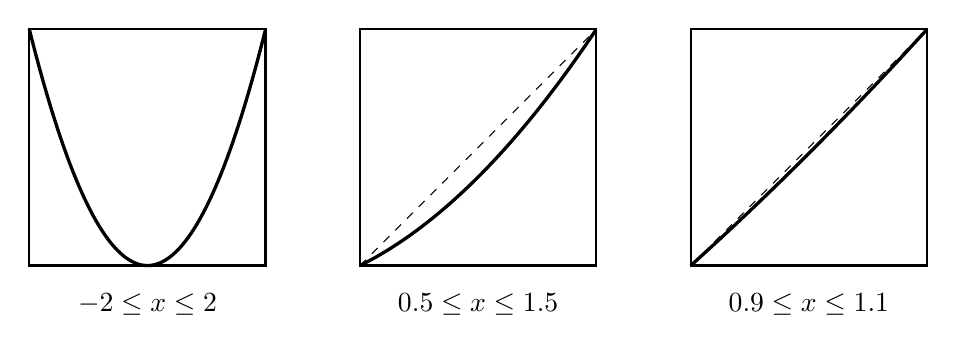
\begin{tikzpicture}[>=stealth]
 \begin{scope}
  \draw[thick] (0,0) rectangle (3,3);
  \draw[very thick,domain=0:1,samples=100,variable=\u]
       plot ({3*\u},{3*((-2+4*\u)*(-2+4*\u))/4});
  \node at (1.5,-0.5) {$-2 \leq x \leq 2$};
 \end{scope}
 \begin{scope}[xshift=4.2cm]
  \draw[thick] (0,0) rectangle (3,3);
  \draw[dashed] (0,0) -- (3,3);
  \draw[very thick,domain=0:1,samples=100,variable=\u]
       plot ({3*\u},{3*(((0.5+\u)*(0.5+\u))-0.25)/2});
  \node at (1.5,-0.5) {$0.5 \leq x \leq 1.5$};
 \end{scope}
 \begin{scope}[xshift=8.4cm]
  \draw[thick] (0,0) rectangle (3,3);
  \draw[dashed] (0,0) -- (3,3);
  \draw[very thick,domain=0:1,samples=100,variable=\u]
       plot ({3*\u},{3*(((0.9+0.2*\u)*(0.9+0.2*\u))-0.81)/0.4});
  \node at (1.5,-0.5) {$0.9 \leq x \leq 1.1$};
 \end{scope}
\end{tikzpicture}
\end{center}

তিনটি ছবিই $y = x^{2}$-এর, কেবল ছবির ফ্রেমের আকার ছোট হতে হতে $(1,1)$ বিন্দুর
চারপাশে গুটিয়ে এসেছে। বাঁয়ে স্পষ্ট বক্ররেখা; ডানে ভাঙা রেখার (সরলরেখা) সঙ্গে
প্রায় মিশে গেছে।

সংখ্যায় দেখা যাক। $x = 1$-এর কাছে
\[
  f(1+h) = (1+h)^{2} = 1 + 2h + h^{2} ,
\]
অর্থাৎ পরিবর্তন $2h + h^{2}$। $h$ ছোট হলে $h^{2}$ পদটি $2h$-এর তুলনায় নগণ্য:
$h = 0.01$-এ $2h = 0.02$ আর $h^{2} = 0.0001$, দুইশ গুণ ছোট। তাই ছোট এলাকায়
$f$ প্রায় রৈখিক, ঢাল $2$।

\begin{idea}[ক্যালকুলাসের কৌশল]
অরৈখিক ফাংশনকে সরাসরি সামলানো কঠিন। কিন্তু প্রতিটি বিন্দুর ক্ষুদ্রাতিক্ষুদ্র পরিসরে তাকে
একটি রৈখিক ফাংশন দিয়ে বদলে দেওয়া যায়, আর ``ক্ষুদ্রাতিক্ষুদ্র পরিসর'' কথাটির নির্ভুল
অর্থ দেয় limit। ওই রৈখিক বদলিটির ঢালই derivative।
\end{idea}

এই বাক্যটাই পরের দুটি অধ্যায়ের সারাংশ। ১৫ নম্বর অধ্যায়ে ঢালটিকে limit দিয়ে
সংজ্ঞায়িত করা হবে, আর ১৬ নম্বরে ওই রৈখিক বদলিটিকেই সরাসরি হাতিয়ার হিসেবে
ব্যবহার করা শেখানো হবে।

\begin{example}
$f(x) = \sqrt{x}$ ফাংশনটি $x = 9$-এর কাছে প্রায় রৈখিক কি না দেখো:
$h = 1$, $h = 0.1$ ও $h = 0.01$-এর জন্য
$\dfrac{f(9+h)-f(9)}{h}$ হিসাব করো।
\end{example}

\begin{solbox}
$f(9) = 3$। এবার
\[
  h = 1: \ \frac{\sqrt{10}-3}{1} \approx 0.16228, \qquad
  h = 0.1: \ \frac{\sqrt{9.1}-3}{0.1} \approx 0.16620 ,
\]
\[
  h = 0.01: \ \frac{\sqrt{9.01}-3}{0.01} \approx 0.16662 .
\]
সংখ্যাগুলো $\dfrac{1}{6} = 0.1\overline{6}$-এর দিকে যাচ্ছে।

বীজগণিতে যাচাই করা যায়। অনুবন্ধী দিয়ে গুণ করে
\[
  \frac{\sqrt{9+h}-3}{h}
  = \frac{(9+h)-9}{h\left( \sqrt{9+h}+3 \right)}
  = \frac{1}{\sqrt{9+h}+3} ,
\]
আর $h \to 0$-এ এটি $\dfrac{1}{3+3} = \dfrac{1}{6}$-এ  যায়। অর্থাৎ $x = 9$-এর
ক্ষুদ্রাতিক্ষুদ্র পরিসরে $\sqrt{x} \approx 3 + \dfrac{h}{6}$, একটি সরলরেখা।
\end{solbox}

\prob{2} \begin{enumerate}
  \item সংখ্যা বসিয়ে দেখাও যে $f(x) = \sqrt{x}$ ও $g(x) = \sin x$ রৈখিক নয়।
  \item নিচের কোনগুলো উপরের কড়া অর্থে রৈখিক: $f(x) = 5x$, $f(x) = 5x+2$,
        $f(x) = x^{2}$?
\end{enumerate}

\begin{sol}
\begin{enumerate}
  \item $a = b = 4$ নিলে $\sqrt{4+4} = \sqrt{8} \approx 2.83$, কিন্তু
        $\sqrt{4}+\sqrt{4} = 4$। সমান নয়।

        $a = b = \tfrac{\pi}{2}$ নিলে $\sin(\pi) = 0$, কিন্তু
        $\sin\tfrac{\pi}{2} + \sin\tfrac{\pi}{2} = 2$। সমান নয়।
  \item $f(x) = 5x$ রৈখিক: $5(x+y) = 5x+5y$ এবং $5(cx) = c \cdot 5x$।

        $f(x) = 5x+2$ রৈখিক নয়: $f(1+1) = 12$, অথচ $f(1)+f(1) = 7+7 = 14$।

        $f(x) = x^{2}$ রৈখিক নয়: $f(1+1) = 4$, অথচ $f(1)+f(1) = 2$।
\end{enumerate}
\end{sol}

\prob{3} $f(x) = x^{2}$-এর জন্য $\dfrac{f(1+h)-f(1)}{h}$ রাশিটি
\begin{enumerate}
  \item $h = 0.1$, $0.01$, $0.001$-এর জন্য হিসাব করো;
  \item বীজগণিত দিয়ে সরল করে $h \to 0$-এ limit নির্ণয় করো;
  \item ব্যাখ্যা করো কেন এখানে $h = 0$ বসানো যেত না, অথচ limit নেওয়া গেল।
\end{enumerate}

\begin{sol}
\begin{enumerate}
  \item $h = 0.1$: $\dfrac{1.21-1}{0.1} = 2.1$;
        $h = 0.01$: $\dfrac{1.0201-1}{0.01} = 2.01$;
        $h = 0.001$: $2.001$। স্পষ্টতই $2$-এর দিকে যাচ্ছে।
  \item $(1+h)^{2} - 1 = 2h + h^{2} = h(2+h)$, তাই $h \neq 0$-এর জন্য
        রাশিটি $2+h$, এবং $h \to 0$-এ limit $2$।
  \item $h = 0$ বসালে রাশিটি $\dfrac{0}{0}$, যা অর্থহীন; ওই একটিমাত্র বিন্দুতে
        ফাংশনটি সংজ্ঞায়িতই নয়। কিন্তু limit-এর সংজ্ঞায় $h$ কখনোই $0$ হয় না,
        তাই $h$ দিয়ে কাটাকাটি করা বৈধ এবং চারপাশের আচরণ থেকে $2$ পাওয়া যায়।

        এটাই ডেরিভেটিভের গোটা ধারণাটির বীজ: যে ভাগফলটি ঠিক ওই বিন্দুতে
        অর্থহীন, তার limit-ই সেখানকার ঢাল। ১৫ নম্বর অধ্যায় এখান থেকেই
        শুরু হবে।
\end{enumerate}
\end{sol}

\end{document}